\documentclass[11pt, a4paper]{article}

\usepackage{color}

\usepackage{amsmath}
\usepackage{amssymb}
\usepackage[pdftex]{graphicx}
\usepackage{alltt}
\usepackage{caption}
\usepackage{subcaption}
\usepackage{epstopdf}
\usepackage{multirow}
\usepackage{placeins}
\usepackage{rotating}




\author{Yacine Derouach, Stefan Hegglin, Huub Heijnen, Elise Ledieu}
\title{Epidemic models of Flu outbreaks}
\begin{document}
\maketitle

\section{Introduction : Model and Data Description}
\label{sec:intro}
\subsection{The SIR model}
\label{sec:SIR}
\paragraph{}
The Susceptible-Infected-Recovered (SIR) model is a deterministic model that describes the influenza transmission. We consider the version proposed by Coehlo et al. \cite{coelho2011bayesian}.

\begin{equation}
\frac{dS}{dt} = - \lambda S
\end{equation}
\begin{equation}
\frac{dI}{dt} = \lambda S - \tau R
\end{equation}
\begin{equation}
\frac{dR}{dt} = \tau R
\end{equation}

with \[ \lambda = \beta (\alpha I + m) \]

where $S$ is the normalized number of susceptible individuals, $I$ is the normalized number of infected individuals, $R$ is the normalized number of recovered individuals, $\tau $ is the recovery rate, $\beta $ is the transmission rate, $\alpha$ is the ratio of symptomatic infection and m is the infectious migration rate.

\begin{figure}[h]
\FloatBarrier
\center
   \includegraphics[width = \textwidth]{figures/picture1.png}
   \caption{Compartmental representation of the SIR model}
   \label{SIRcr}
\end{figure}

$\beta$ is time-dependent and models the seasonality of the flu epidemics. Here, every season is considered as independent of the other ones. The parameters are optimized on a data set only containing winter months, where the epidemy occurs. $\beta$ is here set to 50, as a scaling parameter for the other parameters $\alpha$ and $\tau$.

The set of parameters to be determined in this case is : $ {\alpha, \tau, m, S_o}$. $S_o$ is the number of susceptible individuals at the beginning of each season.

\subsection{The SEIR model}
\paragraph{}
The Susceptible-Exposed-Infected-Recovered (SEIR) model is an extension of the SIR model. We added the Exposed category to the previous system.

\begin{equation}
\frac{dS}{dt} = - \lambda S
\end{equation}
\begin{equation}
\frac{dE}{dt} = \lambda S - \gamma E
\end{equation}
\begin{equation}
\frac{dI}{dt} = \gamma E - \tau R
\end{equation}
\begin{equation}
\frac{dR}{dt} = \tau R
\end{equation}

with \[ \lambda = \beta (\alpha I + m) \]

where $E$ is the normalized number of exposed individuals and $\gamma$ is the transition rate from latent to infected state.

\begin{figure}[h]
\FloatBarrier
\center
   \includegraphics[width = \textwidth]{figures/picture2.png}
   \caption{Compartmental representation of the SEIR model}
   \label{SEIRcr}
\end{figure}

$\beta$ has the same behavior in this model and in the SIR model (Section \ref{sec:SIR}).

The set of parameters to be determined in this model is : $ { \alpha, \gamma, \tau, m, S_0, E_0}$. 

\subsection{Data}
\paragraph{}
The data set used is the one provided by Google Flu Trends. The data is made of the number of infected people reported weekly between December 2011 and May 2014. This time span correspond to three flu seasons. A flu season is considered to begin in December, as the peak of the flu is observed in February in the European countries \cite{baumgartner2012seasonality}. The data was normalized. 

\begin{figure}[h]
\FloatBarrier
\center
   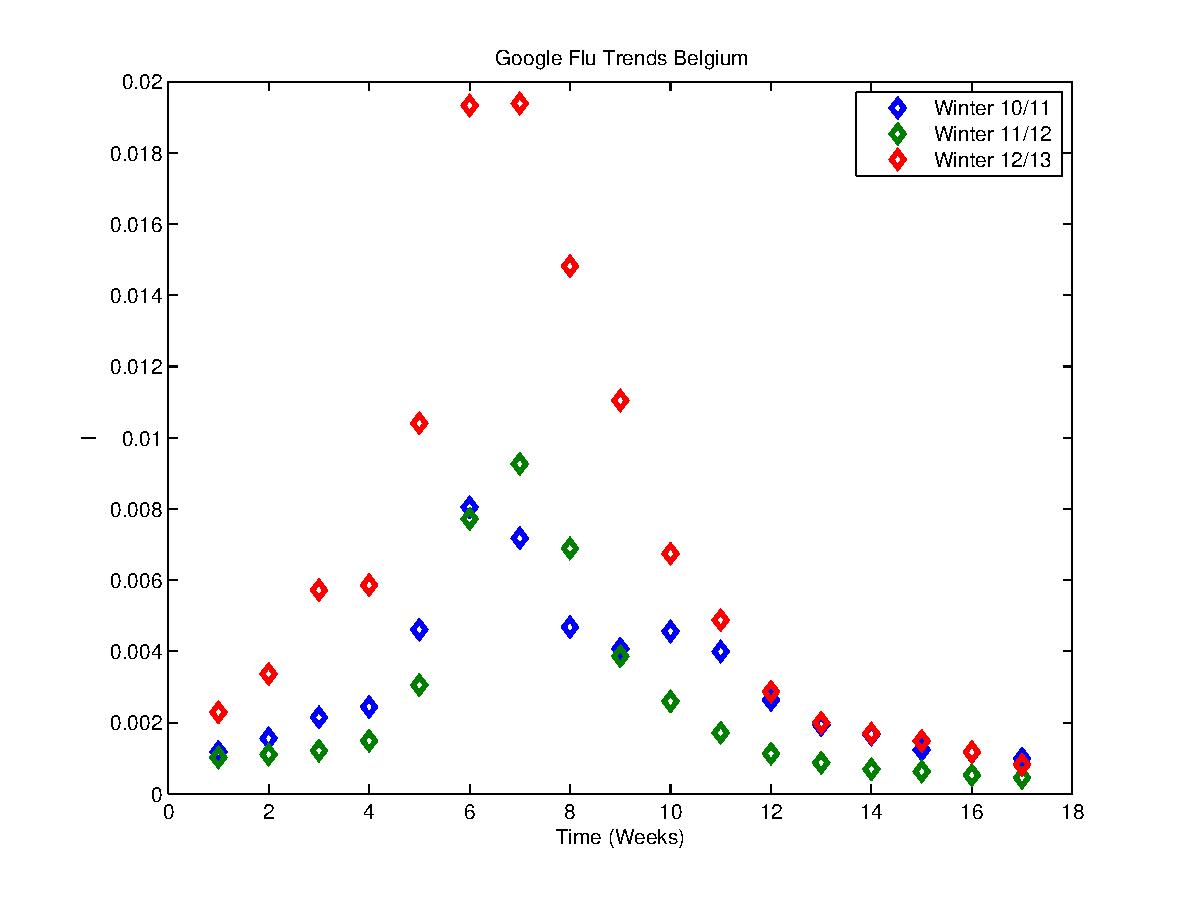
\includegraphics[width = \textwidth]{figures/FluData.eps}
   \caption{Flu Data in Belgium (source : Google Flu Trends)}
   \label{fig:fluData}
\end{figure}

\section{Likelihood}
\paragraph{}
The likelihood of the parameters is 
\begin{equation}
L(\Theta) = L(\Phi) = \prod_{t=1}^T p( d(t) | \Phi(t),I) 
\label{eq:likelihood}
\end{equation}

assuming normal errors with fixed variance $\sigma^2$
\begin{equation}
p(d(t) | \Phi(t),I) = \frac{1}{\sqrt{2\pi}\sigma} \exp^{-\frac{1}{2\sigma^2}[y(t) - I(x(t), \Theta)]}
\label{eq:gaussianPrior}
\end{equation}

where $I(x(t), \Theta)$ is the number of infected people at time $t$ predicted by the model given the input values $x(t)$ ; $y(t)$ is the observed data ; $d(t)$ is the data at a time point.

$I(x(t), \Theta)$ corresponds to the solution of an ODE system. There may be no simple analytical solution for this one and therefore, no analytical derivation possible of it. It depends indeed on the parameter $\beta$, which is time-dependent.

\section{Priors}
\paragraph{}
Thanks to the article by Coehlo et al. \cite{coelho2011bayesian}, it is possible to use informative priors for the SIR model. All of them are defined as uniform on a certain interval.

Here are the priors used for each parameter : 
\begin{itemize}
\item $\alpha \sim \mathcal{U}(0, 0.7)$
\item $\tau \sim \mathcal{U}(0, 5)$
\item $m \sim  \mathcal{U}(0, 1e-4)$
\item $S_0 \sim \mathcal{U}(0, 0.9)$
\end{itemize}

\paragraph{}
In both the SIR and SEIR model, the initial value $I_0$ was chosen to fit the first data point. This determines the value $R_0$ for the SIR model; whereas in the SEIR model an additional parameter $E_0$ has to be infered.

\paragraph{}
We also used uniform priors with lower bound 0 in the SEIR model, however we did not choose any upper bound since we do not want restrict the parameter space unnecessarily.
%\paragraph{}
%Moreover, before computing the Markov Chain Monte Carlo, the initial values of each parameter were optimized. The method used for this prior optimization was a minimum search.

\section{Optimisation and Uncertainty of the parameters}

\subsection{Method : Delayed Rejection Markov Chain Monte Carlo}
\paragraph{}
To find a good parameter fit, two steps were used : first, $\tau$ was fixed to the value $1.4$ as proposed by \cite{coelho2011bayesian} and the other parameters were optimised using Matlab's fminunc(). Then these values were used as initial values for the MCMC sampling process and the constraint for $\tau$ was released. We discarded 2000 samples for burn-in and used 2000 samples for the reconstruction of the posterior.

\subsubsection{Non-zero Migration Rate}
\paragraph{}
The parameters found by the DRAM algorithm are given in table \ref{tab:sirDRAM} for the SIR model and in table \ref{tab:seirDRAM} for the SEIR model.

%\begin{table}[H]
\begin{sidewaystable}[H]
\centering
\begin{tabular}{| c | c | c | c | c | c | c |}
    \hline
    Parameter & Season & Mean (posterior) &  Standard Deviation (posterior) & MPV & uncert MPV & MC error\\ \hline
    \multirow{3}{*}{$\alpha$} & 2010 & 0.19659 & 0.031471 &0.21009 & 0.00028& 0.0061678 \\
    & 2011 & 0.25077 & 0.039664 & 0.27600 & 7.6747e-5 & 0.00777 \\
    & 2012 & 0.094579 & 0.015909 & 0.08250 & 4.6853e-6 & 0.0032257 \\ \hline
    \multirow{3}{*}{$\tau$} & 2010 & 1.4139 & 0.20836 & 1.1549 & 0.1166 & 0.042741 \\ 
    & 2011 & 1.8848 & 0.67187 & 1.5712 & 0.1132 & 0.13294 \\ 
    & 2012 & 1.8732 & 0.33158 & 2.0315 & 0.0761 & 0.068435 \\ \hline
    \multirow{3}{*}{$m$} & 2010 & 3.122e-5 & 2.6057e-5 &7.3915e-5 & 3e-14 & 4.8045e-6 \\ 
    & 2011 & 3.7038e-5 & 3.1233e-5 &1.6678e-5 & 2.99e-14 & 6.663e-6 \\ 
    & 2012 & 3.7222e-5 & 2.6499e-5 & 2.5251e-5 & 5.5e-15 & 5.5581e-6 \\ \hline
    \multirow{3}{*}{$S_o$} & 2010 & 0.17609 & 0.040317 &0.11792 & 0.000572 & 0.0081882 \\
    & 2011 & 0.17968 & 0.079037 & 0.14428 & 0.00022 & 0.015667 \\ 
    & 2012 & 0.53617 & 0.15156 & 0.62491 & 0.00754 & 0.030852 \\ \hline
    \end{tabular}
    \caption{Optimal parameters found for the SIR model in Belgium. MPV denotes the most probable value (mode) of the posterior distribution. The uncertainty around the MPV was computed via numerical computation 2nd derivative of the posterior.}
    \label{tab:sirDRAM}
%\end{table}
\end{sidewaystable}

\paragraph{}
Figures \ref{fig:sir_post1}, \ref{fig:sir_post2} and \ref{fig:sir_post3} sum up the posterior obtained for each season for every parameter in the SIR model. The parameter $m$ seems to be bimodal for each season. For season 2010 and 2011, $\alpha$, $\tau$ and $S_o$ have a unique mode, whereas in the flu season 2012, the distributions are broader, not allowing to establish the existence of one or two clear modes.

\begin{figure}[H!]
\FloatBarrier
\centering
    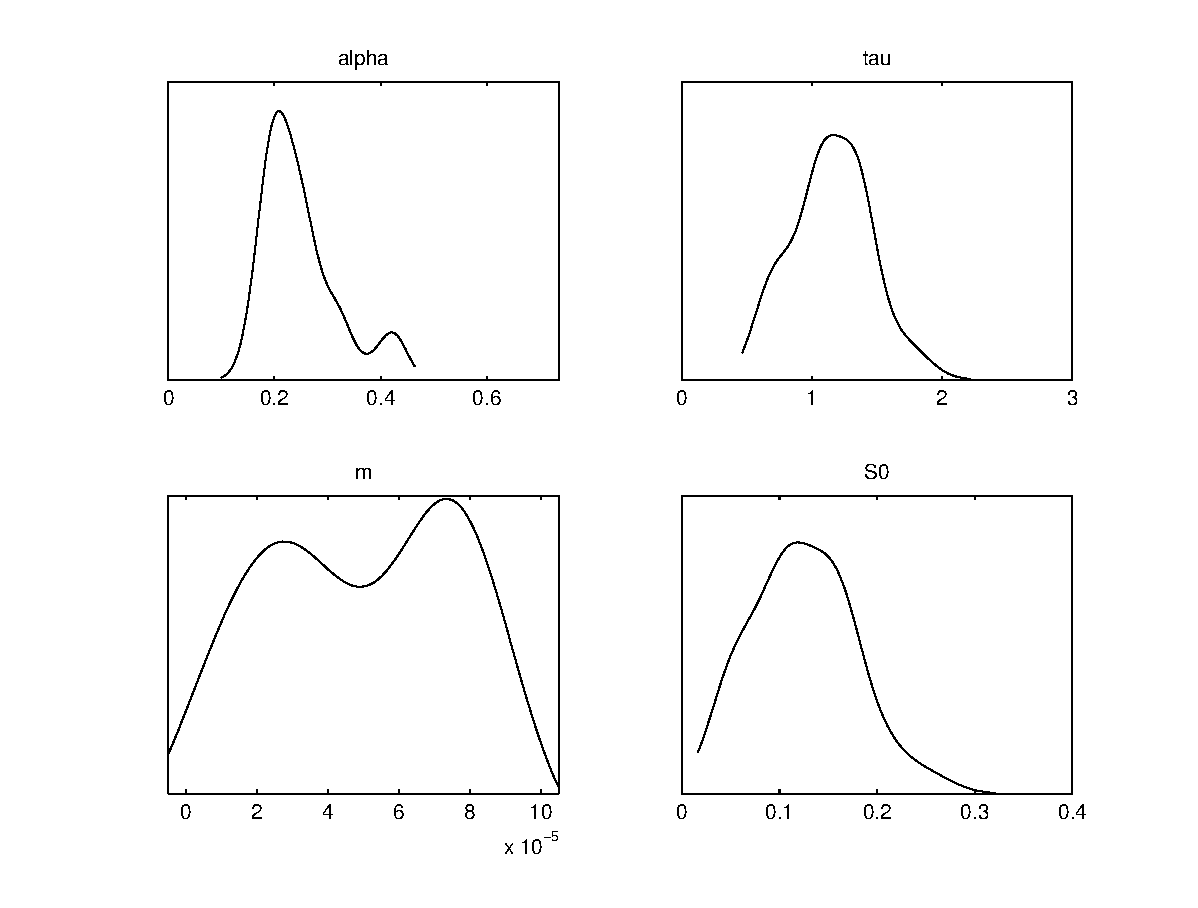
\includegraphics[height = 0.25\textheight]{figures/SIR_posterior_season1.eps}
    \caption{SIR Model : Posterior of each parameter for Season 2010}
    \label{fig:sir_post1}
    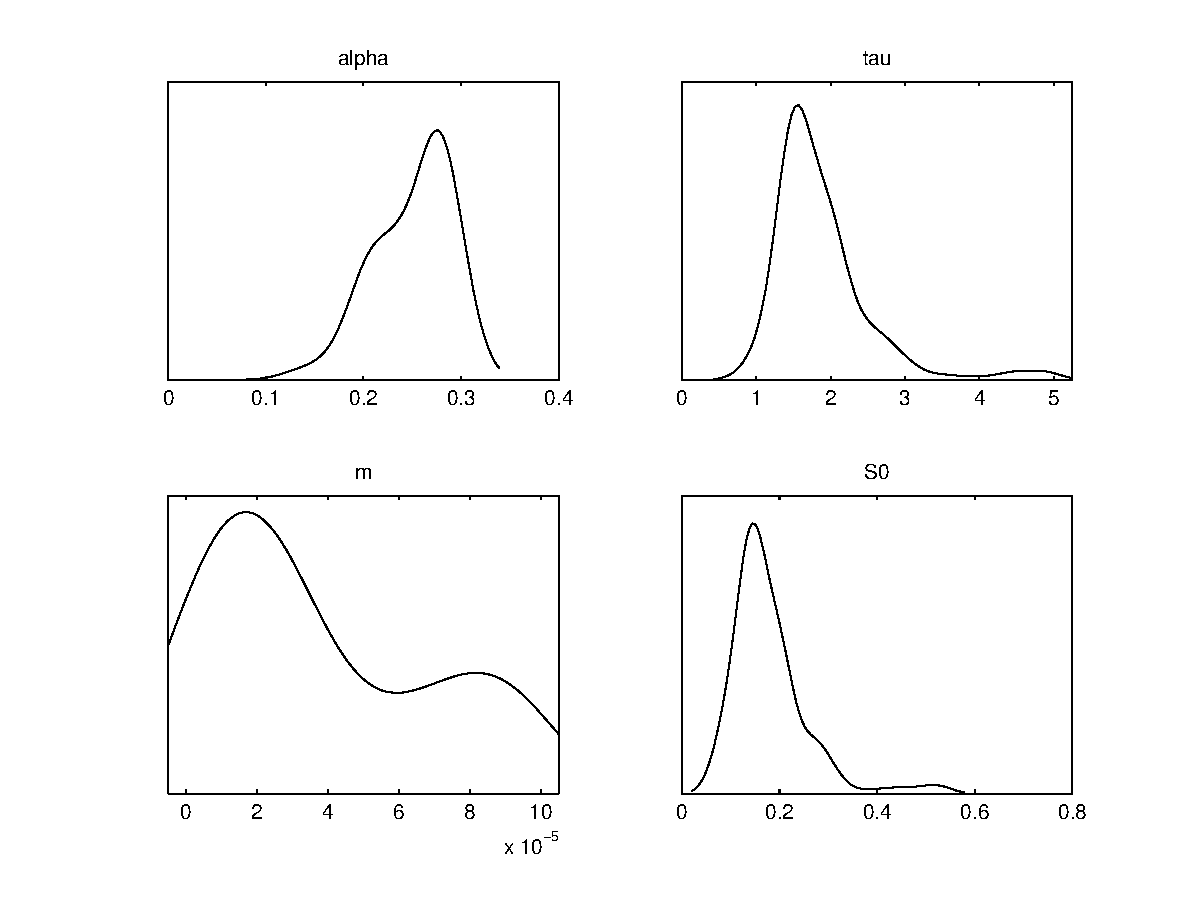
\includegraphics[height = 0.25\textheight]{figures/SIR_posterior_season2.eps}
    \caption{SIR Model : Posterior of each parameter for Season 2011}
    \label{fig:sir_post2}
    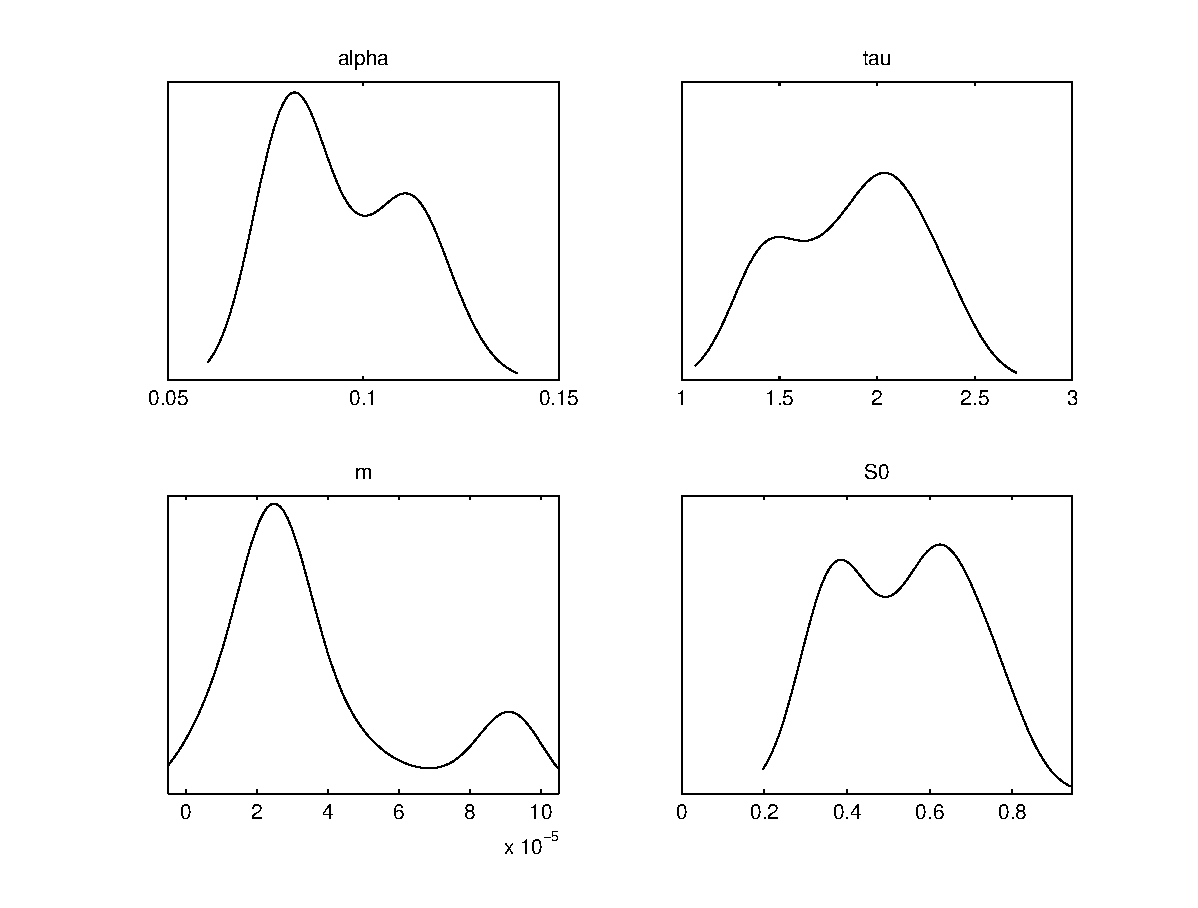
\includegraphics[height = 0.25\textheight]{figures/SIR_posterior_season3.eps}
    \caption{SIR Model : Posterior of each parameter for Season 2012}
    \label{fig:sir_post3}
\end{figure}


\paragraph{}
The following figures \ref{fig:sir_pred1}, \ref{fig:sir_pred2}, \ref{fig:sir_pred3} sum up the prediction obtained by the SIR model for each season. The SIR model for season 2011 shows way more uncertainty in the parameters than for the two other seasons. It might be due to the fact that flu epidemics begin with a delay, compared to the convention adopted in the model definition (Section \ref{sec:intro}).

\begin{figure}[h]
\FloatBarrier
\centering
    \includegraphics[height = 0.25\textheight]{figures/SIR_prediction_season1.eps}
    \caption{SIR Model : Prediction of the SIR Model compared to the Data for Season 2010}
    \label{fig:sir_pred1}
    \includegraphics[height = 0.25\textheight]{figures/SIR_prediction_season2.pdf}
    \caption{SIR Model : Prediction of the SIR Model compared to the Data for Season 2011}
    \label{fig:sir_pred2}
    \includegraphics[height = 0.25\textheight]{figures/SIR_prediction_season3.eps}
    \caption{SIR Model : Prediction of the SIR Model compared to the Data for Season 2012}
    \label{fig:sir_pred3}
\end{figure}


\begin{table}[H]
\FloatBarrier
\centering
\begin{tabular}{| c | c | c | c |}
    \hline
    Parameter & Season & Mean (posterior) &  Standard Deviation (posterior)\\ \hline
    \multirow{3}{*}{$\alpha$} & 2010 & 0.35091 & 0.0040362\\
    & 2011 & 0.9304 & 0.35903\\
    & 2012 & 0.44962 & 0.14712 \\ \hline
    \multirow{3}{*}{$\tau$} & 2010 & 3.8804 & 0.0015877 \\ 
    & 2011 & 14.61 & 6.2934 \\
    & 2012 & 3.3268 & 1.2489\\ \hline
    \multirow{3}{*}{$\gamma$} & 2010 & 1.19999 & 0.00072943\\
    & 2011 & 0.659 & 0.19603 \\ 
    & 2012 & 0.66027 & 0.21565 \\ \hline
    \multirow{3}{*}{$m$} & 2010 & 6.7856e-5 & 6.1501e-5 \\ 
    & 2011 & 6.5738e-6 & 4.3714e-6 \\
    & 2012 & 2.357e-6 & 2.0332e-6 \\ \hline
    \multirow{3}{*}{$S_o$} & 2010 & 0.30925 & 0.0070746 \\ 
    & 2011 & 0.82778 & 0.37533 \\ 
    & 2012 & 0.42712 & 0.17408 \\ \hline
    \multirow{3}{*}{$E_o$} & 2010 & 0.0021444 & 0.0010195\\
    & 2011 & 0.012497 & 0.37533 \\ 
    & 2012 & 0.0080759 & 0.0033979 \\ \hline
    \end{tabular}
    \caption{Infered parameters for the SEIR model in Belgium}
    \label{tab:seirDRAM}
\end{table}

\paragraph{}
The following figures \ref{fig:seir_post1}, \ref{fig:seir_post2} and \ref{fig:seir_post3} sum up the posterior obtained for each season for every parameter in the SEIR model.

\begin{figure}[H!]
\FloatBarrier
\centering
    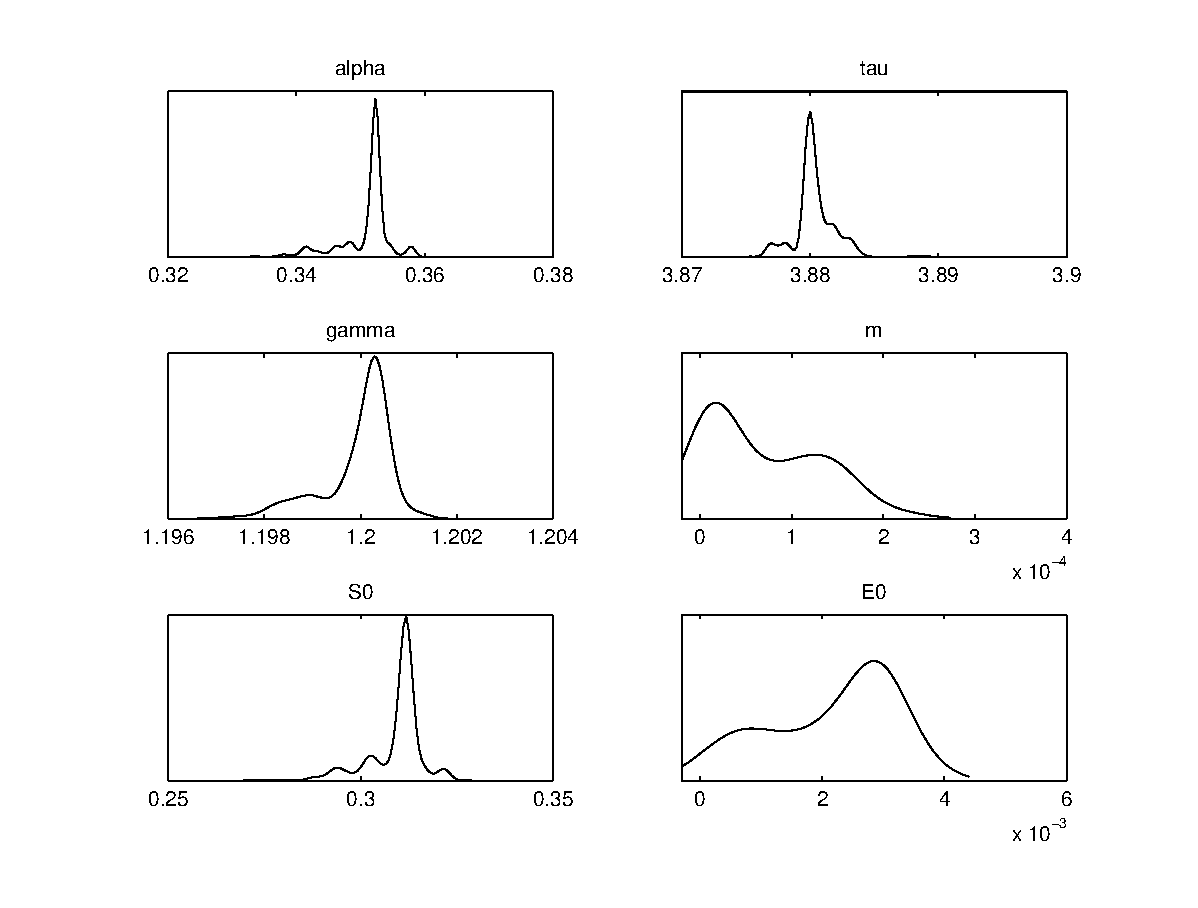
\includegraphics[height = 0.25\textheight]{figures/SEIR_posterior_season1.eps}
    \caption{SEIR Model : Posterior of each parameter for Season 2010}
    \label{fig:seir_post1}
    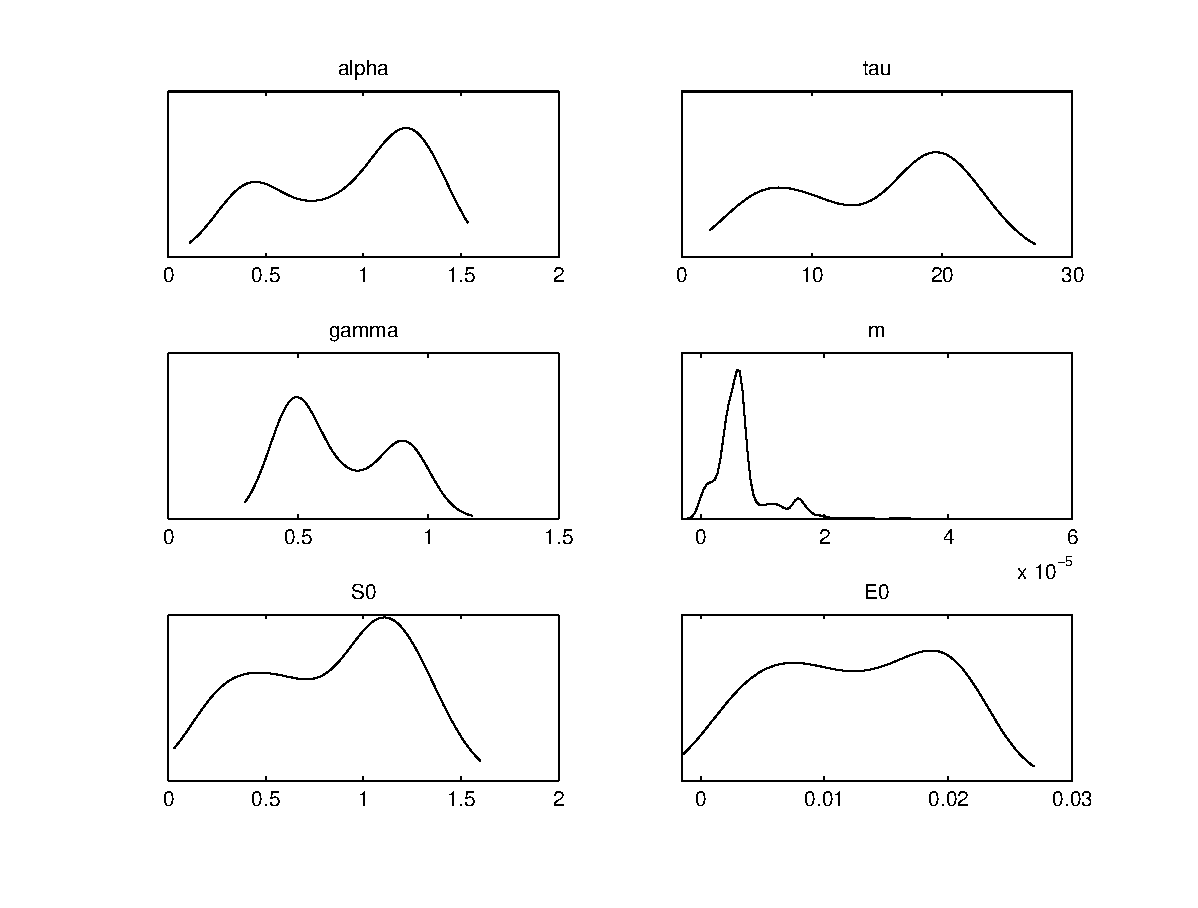
\includegraphics[height = 0.25\textheight]{figures/SEIR_posterior_season2.eps}
    \caption{SEIR Model : Posterior of each parameter for Season 2011}
    \label{fig:seir_post2}
    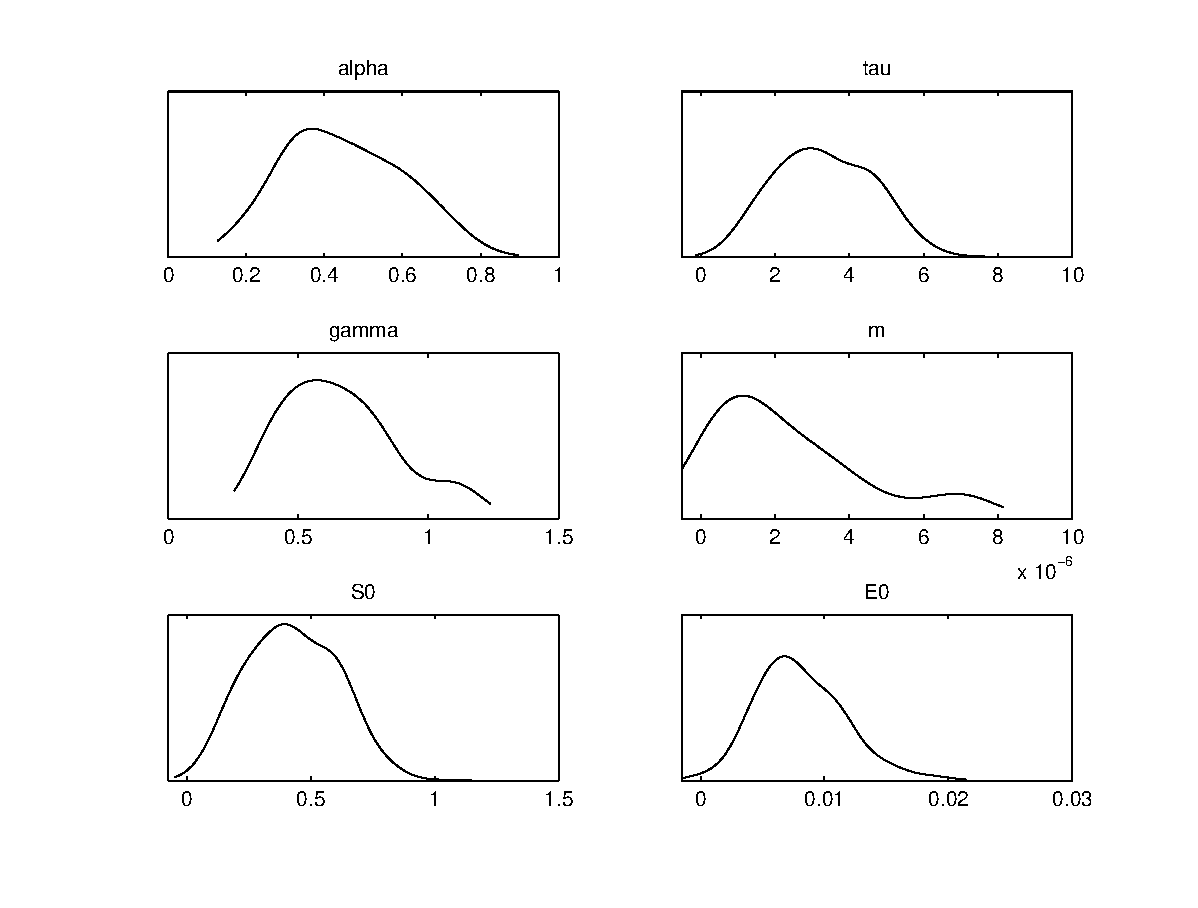
\includegraphics[height = 0.25\textheight]{figures/SEIR_posterior_season3.eps}
    \caption{SEIR Model : Posterior of each parameter for Season 2012}
    \label{fig:seir_post3}
\end{figure}


\paragraph{}
The following figures \ref{fig:seir_pred1}, \ref{fig:seir_pred2}, \ref{fig:seir_pred3} sum up the prediction obtained by the SEIR model for each season.

\paragraph{}
The comparison between the different seasons in the SEIR model are equivalent to the one on the SIR model. The uncertainty of the parameters in the flu season 2011 is well illustrated by the standard deviation linked to the parameter $\tau$, as $\tau$ has a critical influence on the spread of the infection. The characterization of season 2010 is better in the SEIR model than in the SIR model.

\paragraph{}
As the results obtained for the SEIR model and the SIR model are not that different, choosing between the two typically leads to a discussion about the trade-off between accuracy for well-defined data, overall performance for different data sets and number of parameters to fit. As a first approach, using the SIR model gives a general idea of the order of magnitude of the parameters and allows to refine the definition of the data set. For instance, it can answer : Is there a delay in the flu season ?. The SEIR model can then be fitted to have the most accurate model possible. However, the data must be well-defined : it could otherwise lead to a disaster.

\paragraph{}
When we compare the different parameters from one flu season to another in the same model, some season-independent parameters emerge :  $m$ and $tau$ in both models.

\begin{figure}[h]
\FloatBarrier
\centering
    \includegraphics[height = 0.25\textheight]{figures/SEIR_prediction_season1.eps}
    \caption{SEIR Model : Prediction of the SEIR Model compared to the Data for Season 2010}
    \label{fig:seir_pred1}
    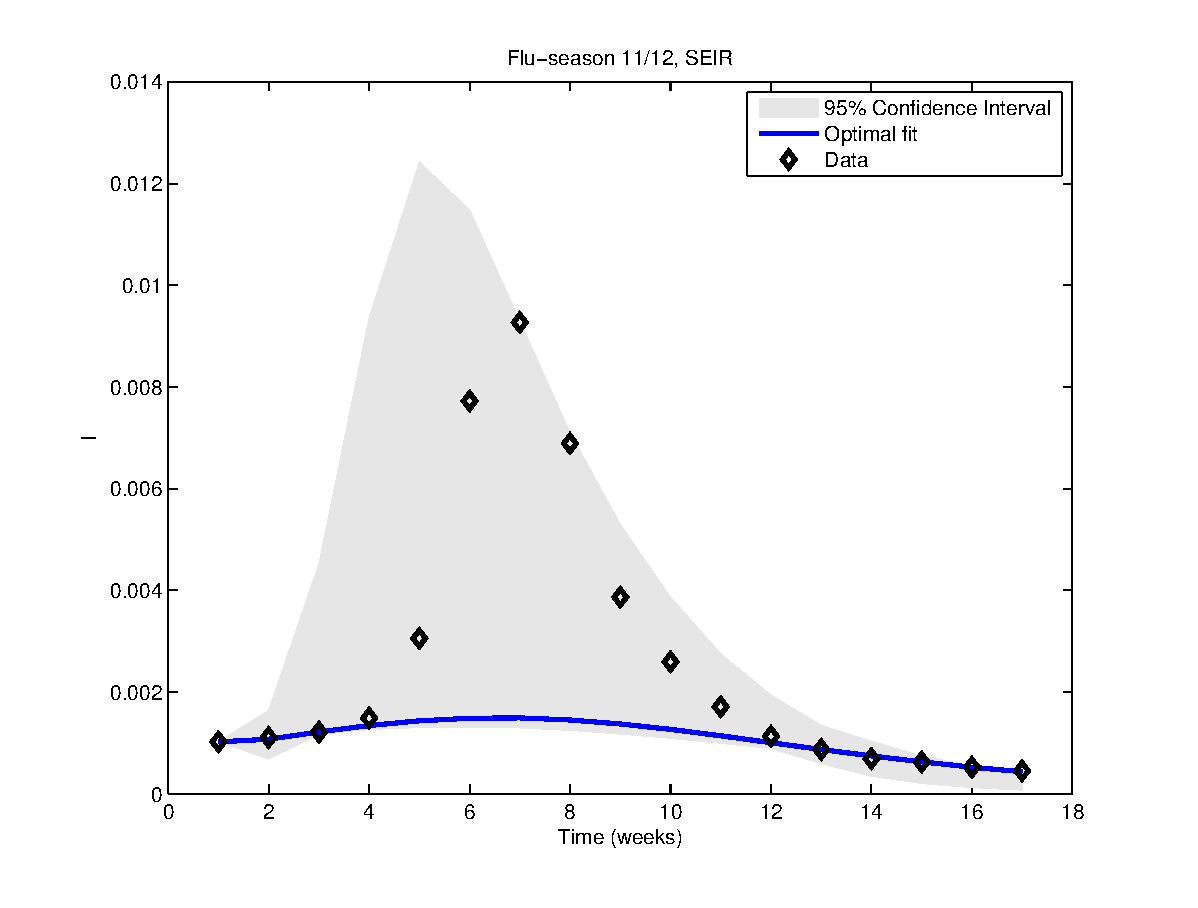
\includegraphics[height = 0.25\textheight]{figures/SEIR_prediction_season2.eps}
    \caption{SEIR Model : Prediction of the SEIR Model compared to the Data for Season 2011}
    \label{fig:seir_pred2}
    \includegraphics[height = 0.25\textheight]{figures/SEIR_prediction_season3.pdf}
    \caption{SEIR Model : Prediction of the SEIR Model compared to the Data for Season 2012}
    \label{fig:seir_pred3}
\end{figure}

\subsubsection{Zero Migration Rate}
\paragraph{}
In Belgium for a zero migration rate, the parameters found by the DRAM algorithm are given in table \ref{tab:sirm0DRAM} for the SIR model
\begin{table}[h]
\FloatBarrier
\centering
\begin{tabular}{| c | c | c | c | c | c |}
    \hline
    Parameter & Season  & Mean &  Standard Deviation & MC error\\ \hline
    \multirow{3}{*}{$\alpha$} & 2010 & 0.19291 & 0.028124 &  0.0055217 \\
    & 2011 & 0.18143 & 0.040817 & 0.0084926 \\
    & 2012 & 0.16 & 0.0.044325 & 0.0079516 \\ \hline
    \multirow{3}{*}{$\tau$} & 2010 & 1.486 & 0.24735 & 0.046956\\ 
    & 2011 & 1.8991 & 0.33592 & 0.07264 \\ 
    & 2012 & 1.2862 & 0.33372 & 0.059622 \\ \hline
    \multirow{3}{*}{$S_o$} & 2010 & 0.19415 & 0.055603 & 0.010885 \\
    & 2011 & 0.23853 & 0.078236 & 0.016589 \\ 
    & 2012 & 0.24848 & 0.11218 & 0.020644 \\ \hline
    \end{tabular}
    \caption{Infered parameters for the SIR model in Belgium with $m=0$}
    \label{tab:sirm0DRAM}
\end{table}



\paragraph{}
The following figures \ref{fig:sir0_post1}, \ref{fig:sir0_post2} and \ref{fig:sir0_post3} sum up the posterior obtained for each season for every parameter in the SIR model.

\paragraph{}
The non migratory model is less accurate than the migratory model. Even if the uncertainty of the parameters is relatively low, it fails to identify the behaviour of the data : for instance, the delay in season 2011 is not taken into account and then it is unable to predict when the peak is going to be.

\begin{figure}[H!]
\FloatBarrier
\centering
    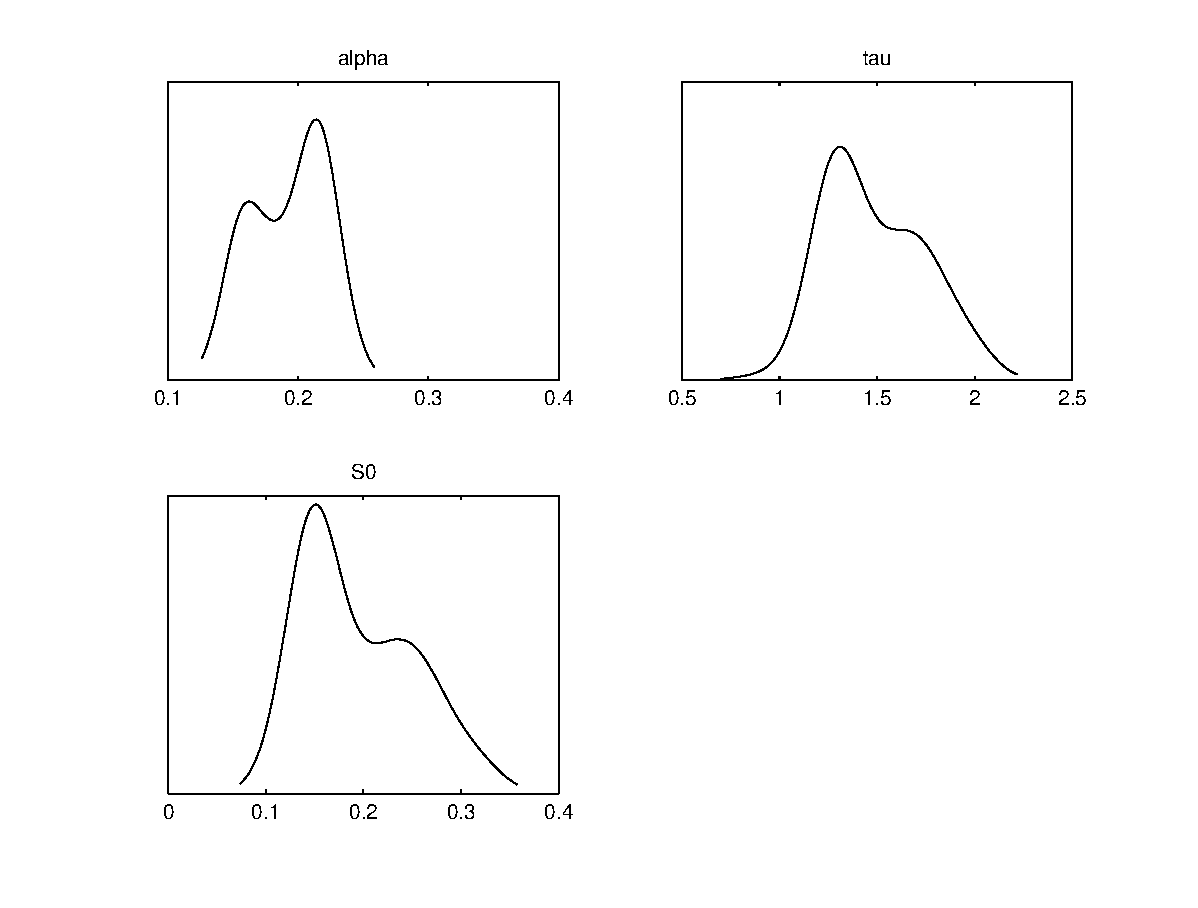
\includegraphics[height = 0.25\textheight]{figures/SIR_posterior_season1_m=0.eps}
    \caption{SIR Model : Posterior of each parameter for Season 2010 with m=0}
    \label{fig:sir0_post1}
    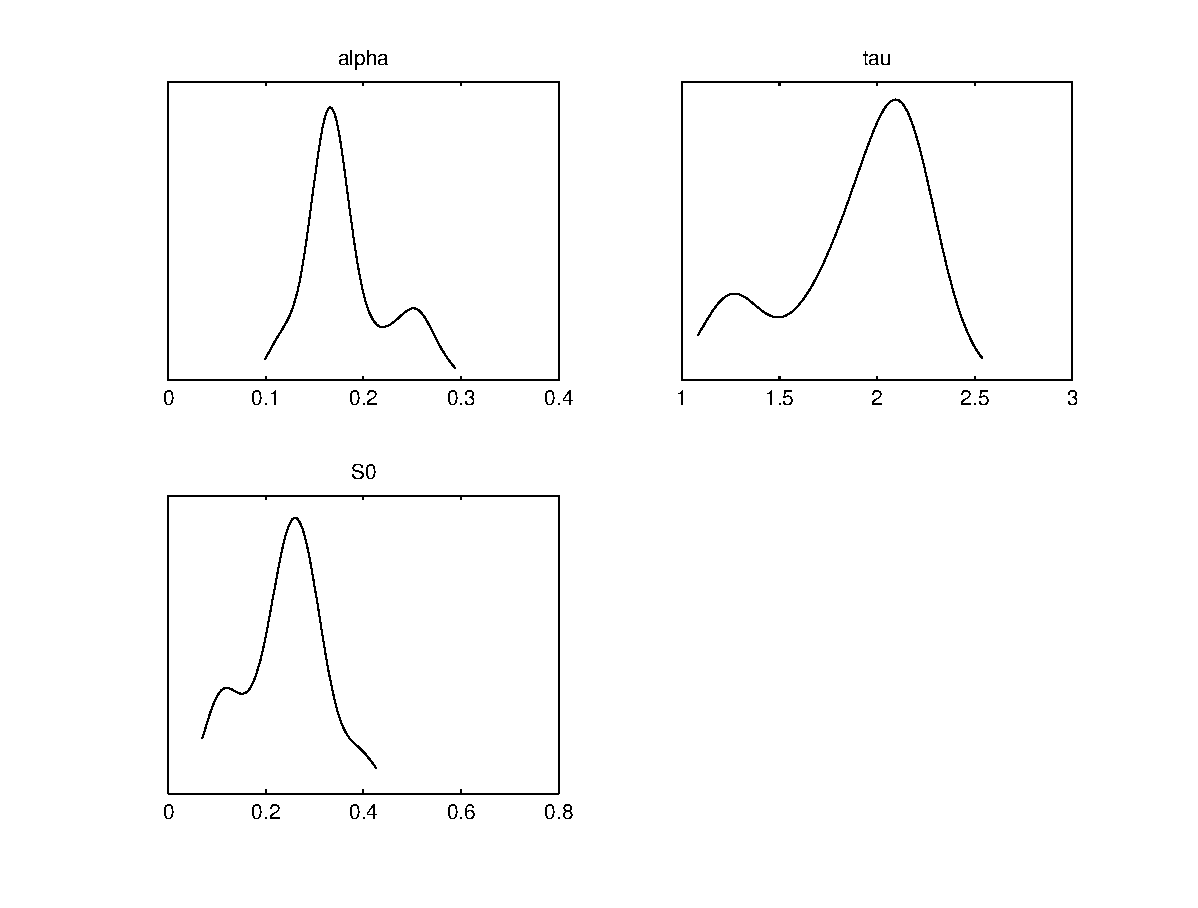
\includegraphics[height = 0.25\textheight]{figures/SIR_posterior_season2_m=0.eps}
    \caption{SIR Model : Posterior of each parameter for Season 2011 with m=0}
    \label{fig:sir0_post2}
    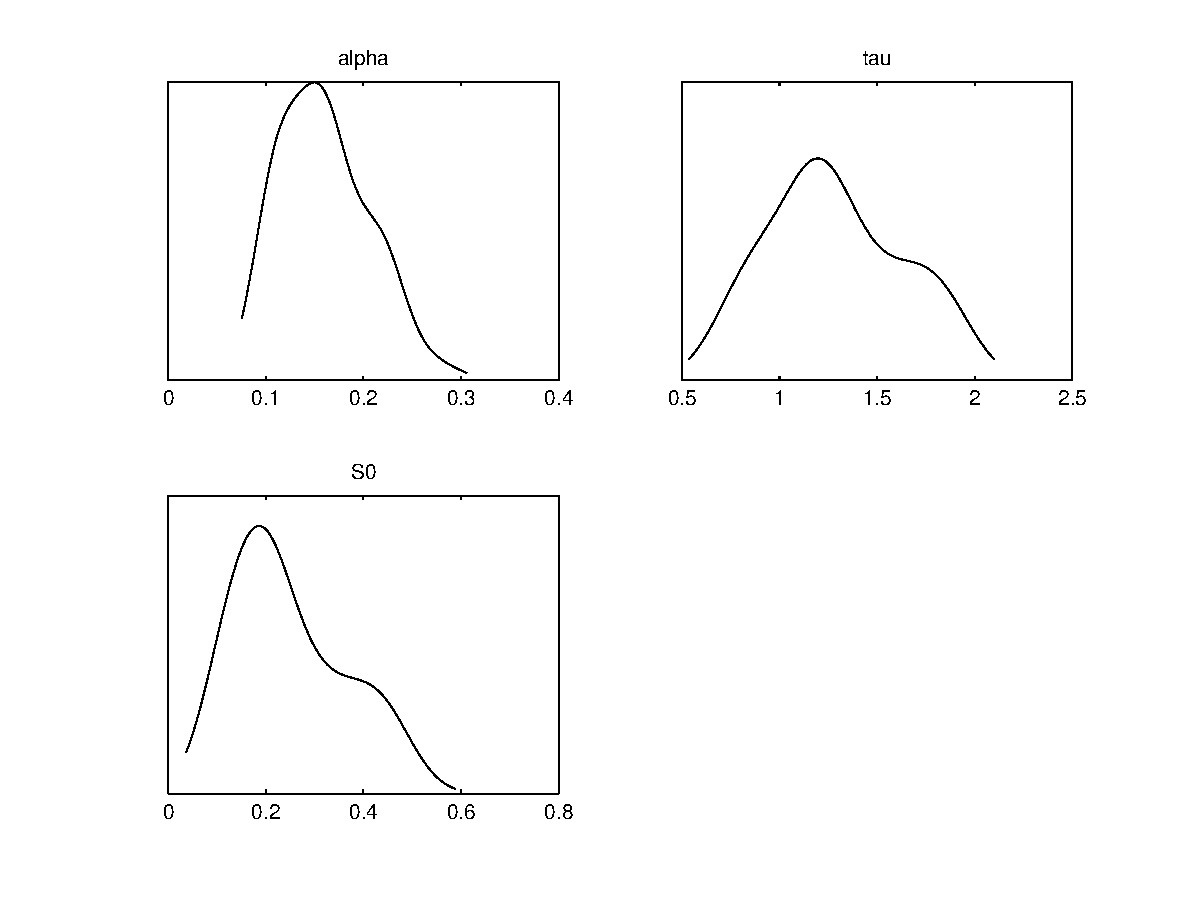
\includegraphics[height = 0.25\textheight]{figures/SIR_posterior_season3_m=0.eps}
    \caption{SIR Model : Posterior of each parameter for Season 2012 with m=0}
    \label{fig:sir0_post3}
\end{figure}


\paragraph{}
The following figures \ref{fig:sir0_pred1}, \ref{fig:sir0_pred2}, \ref{fig:sir0_pred3} sum up the prediction obtained by the SIR model for each season.

\begin{figure}[h]
\FloatBarrier
\centering
    \includegraphics[height = 0.25\textheight]{figures/SIR_prediction_season1_m=0.eps}
    \caption{SIR Model : Prediction of the SIR Model compared to the Data for Season 2010 with m=0}
    \label{fig:sir0_pred1}
    \includegraphics[height = 0.25\textheight]{figures/SIR_prediction_season2_m=0.eps}
    \caption{SIR Model : Prediction of the SIR Model compared to the Data for Season 2011 with m=0}
    \label{fig:sir0_pred2}
    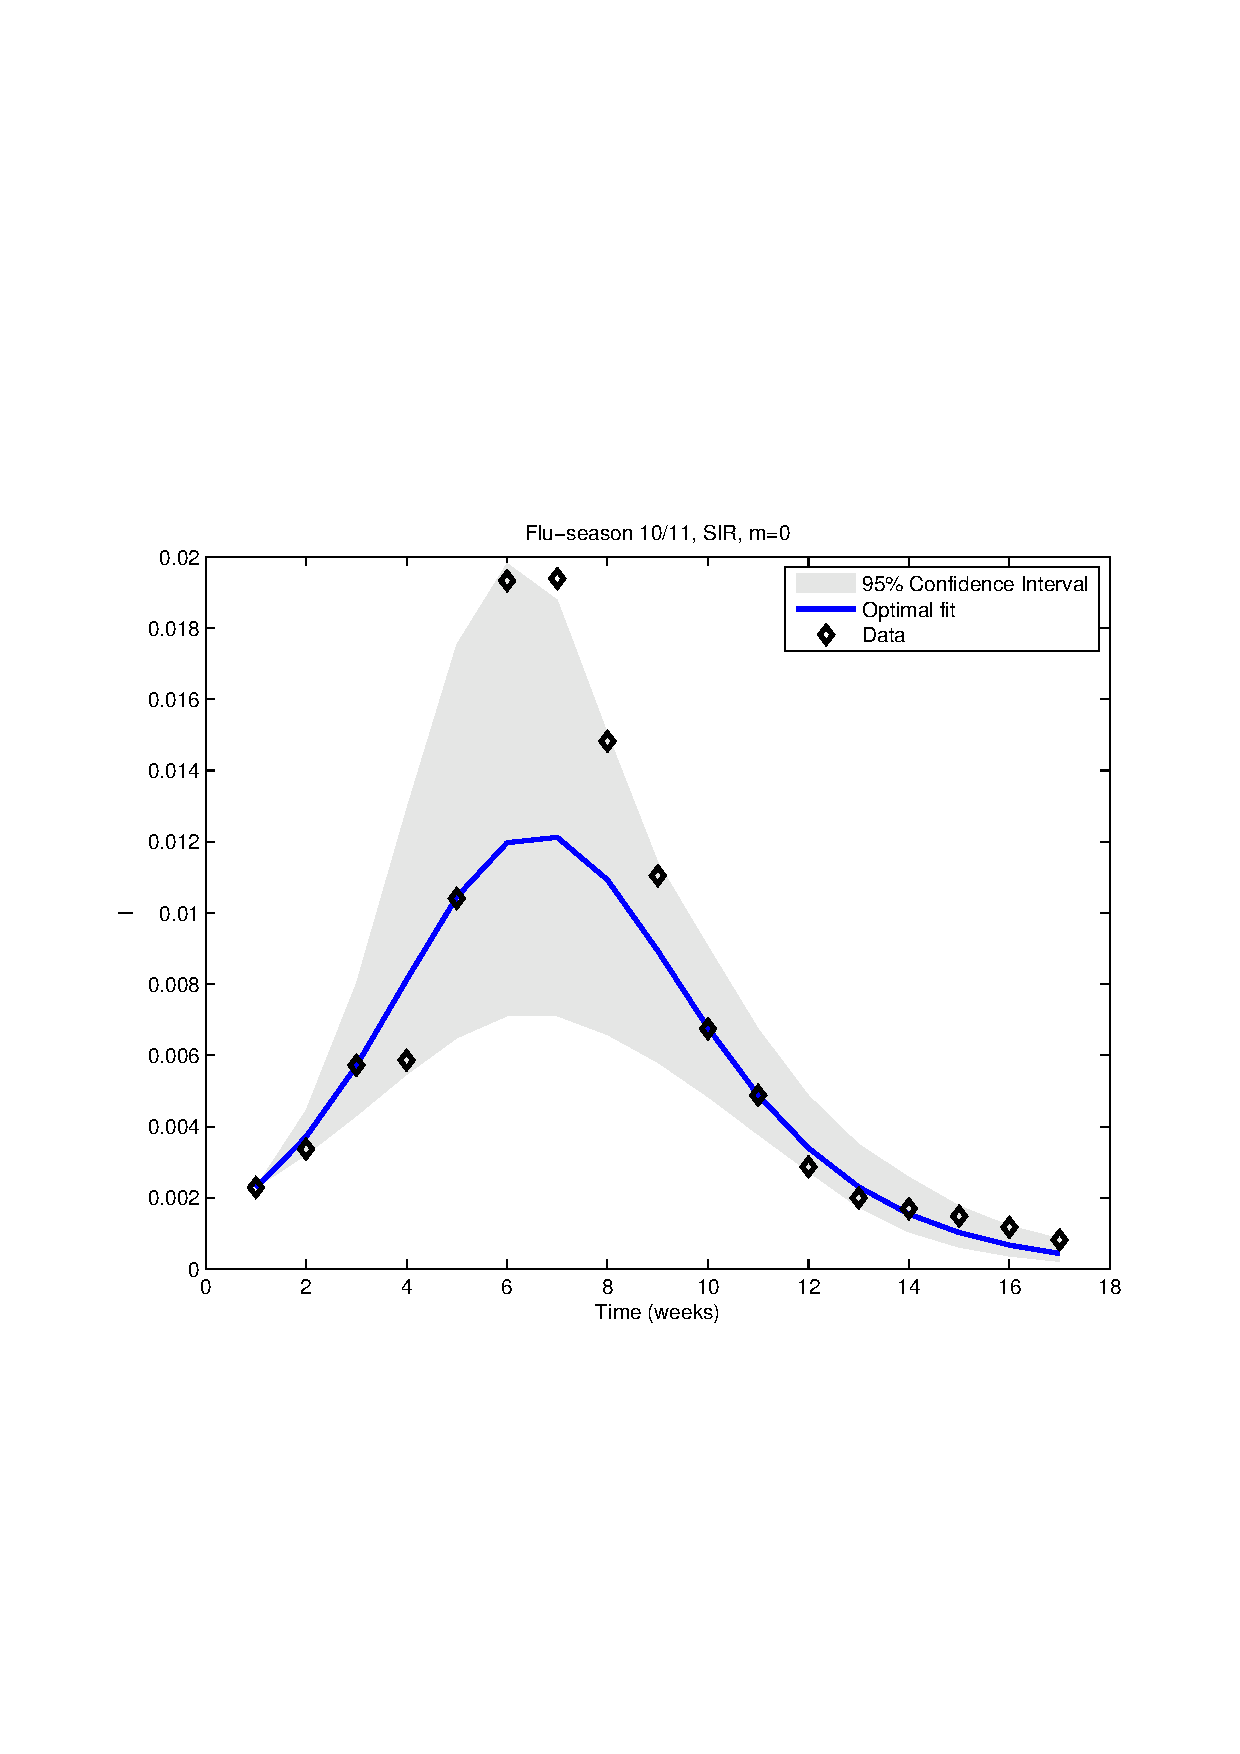
\includegraphics[height = 0.25\textheight]{figures/SIR_prediction_season3_m=0.pdf}
    \caption{SIR Model : Prediction of the SIR Model compared to the Data for Season 2012 with m=0}
    \label{fig:sir0_pred3}
\end{figure}

\subsection{Method : Asymptotic Approximation}
\paragraph{}
Analytically, the Log Posterior function is 

\begin{equation}
l(\Theta) \propto - log(L(\Theta)) - log(\pi(\Theta))
\end{equation}

where $\pi(\Theta)$ is the prior distribution of the parameters.

As gaussian errors are assumed (Equation \ref{eq:gaussianPrior}),

\begin{equation}
l(\Theta) \propto \frac{T}{2} log(\sigma^2) + \frac{1}{2 \sigma^2} \sum_{t=1}^T (y(t)-I(x(t), \Theta))^2 - log(\pi(\Theta))
\end{equation}

The best estimate can thus be derived by $\frac{\partial l}{\partial \Theta}(\Theta^*) = 0$. The following formula is then obtained :

\begin{equation}
\sum_{t=1}^T (y(t) - I(x(t), \Theta^*)) \frac{\partial I(x(t), \Theta^*)}{\partial \Theta} = 0
\end{equation}

The optimal model parameters can be retrieved by solving a least square optimization problem. 

The spread of uncertainty is modelled by the inverse of the Hessian :

\begin{equation}
H(\Theta^*) = \frac{\partial^2 l}{\partial \Theta^2} (\Theta^*) 
\end{equation}

As there is no analytical formulation of the solution $I(x(t), \Theta)$, we solved the optimisation task using Matlab's fminsearch optimiser, see tables \ref{tab:sir}, \ref{tab:sir0} and \ref{tab:seir}. The numerical computation of the full Hessian failed, indicating a very unstable optimum. This is not surprising, because the ODEs are very sensitive with respect to the parameters and the parameters span different orders of magnitude.


%\begin{table}[H]
%\FloatBarrier
%\centering
%\begin{tabular}{| c | c | c |}
%    \hline
%    Parameter & Season  & Optimal value\\ \hline
%    \multirow{3}{*}{$\alpha$} & 2010 &0.227 \\
%    & 2011 & 0.283\\
%    & 2012 & 0.126 \\ \hline
%    \multirow{3}{*}{$\tau$ (fixed)} & 2010 & 1.4\\ 
%    & 2011 & 1.4\\ 
%    & 2012 & 1.4 \\ \hline
%    \multirow{3}{*}{$m$} & 2010 & 3.3e-6\\ 
%    & 2011 & 4.1e-6\\
%    & 2012 & 2.6e-6\\ \hline
%    \multirow{3}{*}{$S_o$} & 2010 & 0.162\\
%    & 2011 & 0.136 \\ 
%    & 2012 & 0.310 \\ \hline
%    \end{tabular}
%    \caption{Optimal parameters found by optimisation using fminunc() for the SIR model in Belgium}
%    \label{tab:optimVals}
%\end{table}
%
%\begin{table}[H]
%\FloatBarrier
%\centering
%\begin{tabular}{| c | c | c |}
%    \hline
%    Parameter & Season  & Optimal value\\ \hline
%    \multirow{3}{*}{$\alpha$} & 2010 &0.230 \\
%    & 2011 & 0.289\\
%    & 2012 & 0.126 \\ \hline
%    \multirow{3}{*}{$\tau$ (fixed)} & 2010 &1.4 \\ 
%    & 2011 & 1.4\\ 
%    & 2012 & 1.4 \\ \hline
%    \multirow{3}{*}{$S_o$} & 2010 & 0.160\\
%    & 2011 & 0.134 \\ 
%    & 2012 & 0.312 \\ \hline
%    \end{tabular}
%    \caption{Optimal parameters found by optimisation using fminunc() for the SIR m=0 model in Belgium}
%    \label{tab:optimValsm0}
%\end{table}
%
%
%\begin{table}[H]
%\FloatBarrier
%\centering
%\begin{tabular}{| c | c | c |}
%    \hline
%    Parameter & Season & Optimal value\\ \hline
%    \multirow{3}{*}{$\alpha$} & 2010 & 0.311\\
%    & 2011 & 0.839\\
%    & 2012 & 0.352 \\ \hline
%    \multirow{3}{*}{$\tau$} & 2010 & 1.858 \\ 
%    & 2011 & 3.524\\
%    & 2012 & 2.174\\ \hline
%    \multirow{3}{*}{$\gamma$} & 2010 & 2.303\\
%    & 2011 & 0.584\\ 
%    & 2012 & 0.702\\ \hline
%    \multirow{3}{*}{$m$} & 2010 & 2.2e-6\\ 
%    & 2011 & 2.1e-6\\
%    & 2012 & 2.4e-6 \\ \hline
%    \multirow{3}{*}{$S_o$} & 2010 &0.171 \\ 
%    & 2011 & 0.112 \\ 
%    & 2012 & 0.287\\ \hline
%    \multirow{3}{*}{$E_o$} & 2010 & 0.001\\
%    & 2011 & 0.006\\ 
%    & 2012 & 0.008\\ \hline
%    \end{tabular}
%    \caption{Optimal parameters found by optimisation using fminunc() for the SEIR model in Belgium}
%    \label{tab:optimValsSEIR}
%\end{table}




\begin{table}[H]
\FloatBarrier
\centering
\begin{tabular}{| c | c | c |}
    \hline
    Parameter & Season & Optimal Value \\ \hline
    \multirow{3}{*}{$\alpha$} & 2010 & 0.227\\
    & 2011 & 0.283\\
    & 2012 & 0.126 \\ \hline
    \multirow{3}{*}{$\tau$ (fixed)} & 2010 & 1.4 \\ 
    & 2011 & 1.4\\
    & 2012 & 1.4\\ \hline
    \multirow{3}{*}{$m$} & 2010 & 3.3e-6\\ 
    & 2011 & 4.1e-6 \\
    & 2012 & 2.6e-6 \\ \hline
    \multirow{3}{*}{$S_o$} & 2010 & 0.162 \\ 
    & 2011 & 0.136 \\ 
    & 2012 & 0.31 \\ \hline
    \end{tabular}
    \caption{Most probable value of the parameters in the SIR model found by fminsearch()}
    \label{tab:sir}
\end{table}

\begin{table}[H]
\FloatBarrier
\centering
\begin{tabular}{| c | c | c |}
    \hline
    Parameter & Season & Optimal Value \\ \hline
    \multirow{3}{*}{$\alpha$} & 2010 & 0.23\\
    & 2011 & 0.289\\
    & 2012 & 0.126 \\ \hline
    \multirow{3}{*}{$\tau$ (fixed) } & 2010 & 1.4 \\ 
    & 2011 & 1.4\\
    & 2012 & 1.4\\ \hline
    \multirow{3}{*}{$S_o$} & 2010 & 0.16 \\ 
    & 2011 & 0.134 \\ 
    & 2012 & 0.312 \\ \hline
    \end{tabular}
    \caption{Most probable value of the parameters in the SIR model with $m=0$ found by fminsearch()}
    \label{tab:sir0}
\end{table}


\begin{table}[H]
\FloatBarrier
\centering
\begin{tabular}{| c | c | c |}
    \hline
    Parameter & Season & Optimal Value \\ \hline
    \multirow{3}{*}{$\alpha$} & 2010 & 0.311\\
    & 2011 & 0.839\\
    & 2012 & 0.352 \\ \hline
    \multirow{3}{*}{$\tau$} & 2010 & 1.858 \\ 
    & 2011 & 3.524\\
    & 2012 & 2.174\\ \hline
    \multirow{3}{*}{$\gamma$} & 2010 & 2.303 \\ 
    & 2011 & 0.584\\
    & 2012 & 0.702\\ \hline
    \multirow{3}{*}{$m$} & 2010 & 2.2e-6\\ 
    & 2011 & 2.1e-6 \\
    & 2012 & 2.4e-6 \\ \hline
    \multirow{3}{*}{$S_o$} & 2010 & 0.171 \\ 
    & 2011 & 0.112 \\ 
    & 2012 & 0.287 \\ \hline
    \multirow{3}{*}{$E_o$} & 2010 & 0.001 \\ 
    & 2011 & 0.006 \\ 
    & 2012 & 0.008 \\ \hline
    \end{tabular}
    \caption{Most probable value of the parameters in the SEIR model found by fminsearch()}
    \label{tab:seir}
\end{table}



\section{Conclusion}
The parameter inference of both the SIR and SEIR models were performed using Delayed Rejection Markov Chain Monte Carlo. Results similar to \cite{coelho2011bayesian} were obtained and show some consistency with a possible physical interpretation. It is noticeable that the parameters don't change between the migratory and the non-migratory model. Even though the parameter uncertainty is rather small, the posterior prediction of the infected rate showed a large uncertainty; the models are very sensitive. Possible improvements could be achieved by using more data or a bigger sample size to reconstruct the posterior.







\bibliographystyle{plain}
\bibliography{references.bib}

\end{document}
